\documentclass[fleqn,a4paper,12pt]{article}

%used Packages
\usepackage{standalone}		% Zum Einlesen aus anderen .tex-Files
\usepackage{geometry}		% Zur Bearbeitung des Layouts (Ränder,...)
\usepackage[german]{babel}
\usepackage[utf8]{inputenc}
\usepackage{amsmath}		% Mathematische Symbole
\usepackage{amssymb}     	% Nochmehr mathematische Symbole
\usepackage{dsfont}      	% Schriftsatz fuer Zahlenmengensymbole
%\usepackage{verbatim}   	% erweiterte Verbatim-Umgebung
\usepackage{alltt}       	% Quasi-Verbatim-Umgebung
\usepackage{fancyhdr}    	% Eigene Kopfzeilen
\usepackage{graphicx}    	% Zum Einbinden von Grafiken
							% Einbinden einer eps-Grafik geht so: includegraphics{path}
\usepackage{wrapfig}
\usepackage{lscape}
\usepackage{rotating}
\usepackage{epstopdf}

% Skalierung der Grafiken
\setlength{\unitlength}{1cm}

\frenchspacing               % Kein Extrafreiraum nach Satzzeichen
\setlength{\parindent}{0pt}  % Neue Absaetze nicht einruecken
%\sloppy                     % Schlampige Absatzformatierung
\fussy                       % Penible Absatzformatierung
\linespread{1.5}             % Zeilenabstand


% Seitenraender
\geometry{left=30mm, right=40mm, bottom=30mm}
				% Doc-class, Packageimports, fancy stuff
%Seitenränder formatieren
\addtolength{\voffset}{-2cm}
\addtolength{\textheight}{0cm}
\addtolength{\hoffset}{0cm}
\addtolength{\textwidth}{2cm}
\addtolength{\headheight}{2cm} % fuer jeden Strichkode einen Zentimeter

% Font fuer Code 39
\font\xlix=wlc39 scaled 1200
\newcommand\barcode[1]{{\xlix@#1@}}

% Name, Matrikelnummer, Barcode
\newcommand\student[2]{
	\mbox{\scriptsize
		\begin{tabular}{@{}l@{}r@{}}
			\multicolumn{2}{@{}r@{}}{\barcode{#2}}\\
			#1&#2\\
		\end{tabular}}}

% Kopfzeile
\pagestyle{fancy}            % Eigene Kopfzeilen verwenden
\lhead{
	\small
	\textsc{Grundlagen der Signalverarbeitung \\
		WS 2017/2018 \\
		\"Ubung (\today)}
	\vfill}
\rhead{
	\begin{tabular}[b]{@{}rr@{}}
		\student{Philipp Badenhoop}{572693} &
		\student{Steven Lange}{568733} \\
		\student{Pascal Jochmann}{575056} &
		\student{Kevin Trogant}{572451}
\end{tabular}}			% Definition der Kopfzeile
%andere Definitionen
\providecommand{\R}{{\mathbb R}}
\providecommand{\N}{{\mathbb N}}
\providecommand{\Z}{{\mathbb Z}}
\providecommand{\Q}{{\mathbb Q}}
\providecommand{\C}{{\mathbb C}}
\providecommand{\F}{\mathcal{F}}
\providecommand{\less}{\setminus}
\providecommand{\inv}{{}^{-1}}
\providecommand{\Land}{\bigwedge}
\providecommand{\Lor}{\bigvee}			% Liste der zusätzlichen Commands und redefines

\begin{document}
	\section*{Übungsaufgabe 44:}

	\begin{tabular}{|c|c|c|}
		\hline
		Rechenweg & Rechenzeit [s] & relativ zur FFT \\ \hline
		DFT ohne Zuteilung & 83.79 & 299256x \\ \hline
		DFT mit Zuteilung & 31.63 & 112970x \\ \hline
		FFT & 0.00028 & 1x \\ \hline
	\end{tabular}
	
\newpage
	\section*{Übungsaufgabe 45:}
		Sei $x_1(t):\R \to \{0,1\}, t\mapsto 1_{[0,1]}(t)$  und $x_2(t) = \frac{1}{2}t\cdot 1_{[0,1]}(t)$, wobei in $x_1$ und $x_2$ $1_{[0,1]}$ die Standard-Indikatorfunktion ist. Für ein bel. Intervall $I\subset\R$  gilt: $1_{I}(t) = \begin{cases} 1, &\text{wenn } t\in I\\ 0, & \text{sonst.}\end{cases}$.
		
		Sei weiter $h:\R\times\R \to \R$ wie folgt definiert:
		$$h(t,\tau) = x_1(t)\cdot x_2(t+\tau) = 1_{[0,1]}\cdot\frac{1}{2}(t+\tau)\cdot1_{[0,1]}(t+\tau)$$
		Es gilt $1_{[0,1]}(t+\tau) = 1_{[-\tau,1-\tau]}(t)$ sowie:
		$$1_{[0,1]}(t)\cdot1_{[-\tau,1-\tau]}(t) = 1_{[0,1]\cap[-\tau,1-\tau]}(t) := \begin{cases}
		1_{\emptyset}(t) = 0,	& \text{falls } -\infty < \tau < -1\\
		1_{[-\tau,1]}(t),		& \text{falls } -1 \le \tau < 0\\
		1_{[0,1-\tau]}(t),		& \text{falls } 0 \le \tau \le 1\\
		1_{\emptyset}(t) = 0,	& \text{falls } 1 < \tau < \infty
		\end{cases}$$
		Es gilt also $h(t,\tau) = \left(\frac{1}{2}t +\frac{1}{2}\tau\right) \cdot 1_{[0,1]\cap[-\tau,1-\tau]}(t)$.\\
		Sei weiter $k:\R\to\R$ mit dem Standard-Lebesgue-Maß wie folgt definiert:
		$$k(\tau) = \int_\R h(t,\tau)\lambda(dt)= \int_{[0,1]\cap[-\tau,1-\tau]}\frac{1}{2}t+\frac{1}{2}\tau\lambda(dt)$$
		\begin{tabular}{r | c c | c}
			$\tau$	&	$\int_{[0,1]\cap[-\tau,1-\tau]}\frac{1}{2}t\lambda(dt)$ & $\frac{1}{2}\tau\cdot\int_{[0,1]\cap[-\tau,1-\tau]}1\lambda(dt)$&	$k(\tau)$\\
			\hline
			$-2.00$	&	0.000	&	 0.000	&	 0.000	\\
			%$-1.50$	&	 0.0	&	 0.0	&	 0.0	\\
			$-1.00$	&	0.000	&	 0.000	&	0.000	\\
			$-0.75$	&	0.109	&	-0.094	&	0.015\\
			$-0.50$	&	0.188	&	-0.125	&	0.063\\
			$-0.25$	&	0.234	&	-0.094	&	0.140\\
			$ 0.00$	&	0.250	&	 0		&	0.250\\
			$ 0.25$	&	0.141	&	 0.094	&	0.235\\
			$ 0.50$	&	0.063	&	 0.125	&	0.188\\
			$ 0.75$	&	0.016	&	 0.094	&	0.110\\
			$ 1.00$	&	0.000	&	 0.000	&	0.000\\
			%$ 1.5$	&	\\
			$ 2.00$	&	0.000	&	 0.000	&	 0.000\\
		\end{tabular}\\
	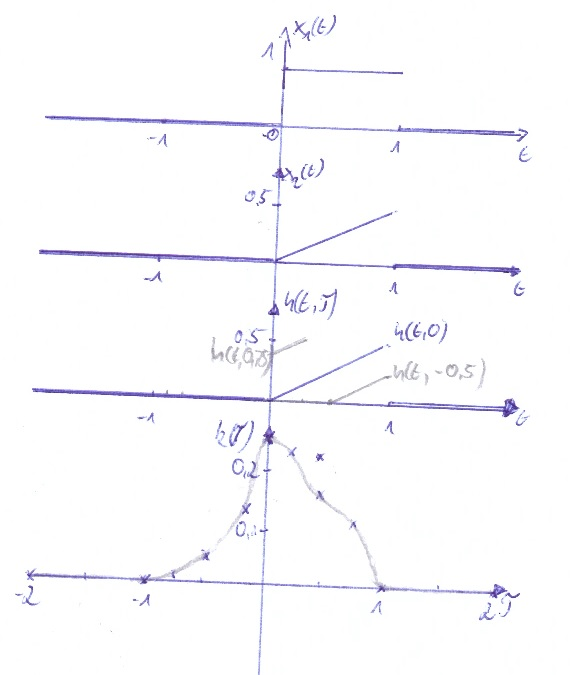
\includegraphics[angle=2]{A45_graph.png}
\newpage
	\section*{Übungsaufgabe 46:}

	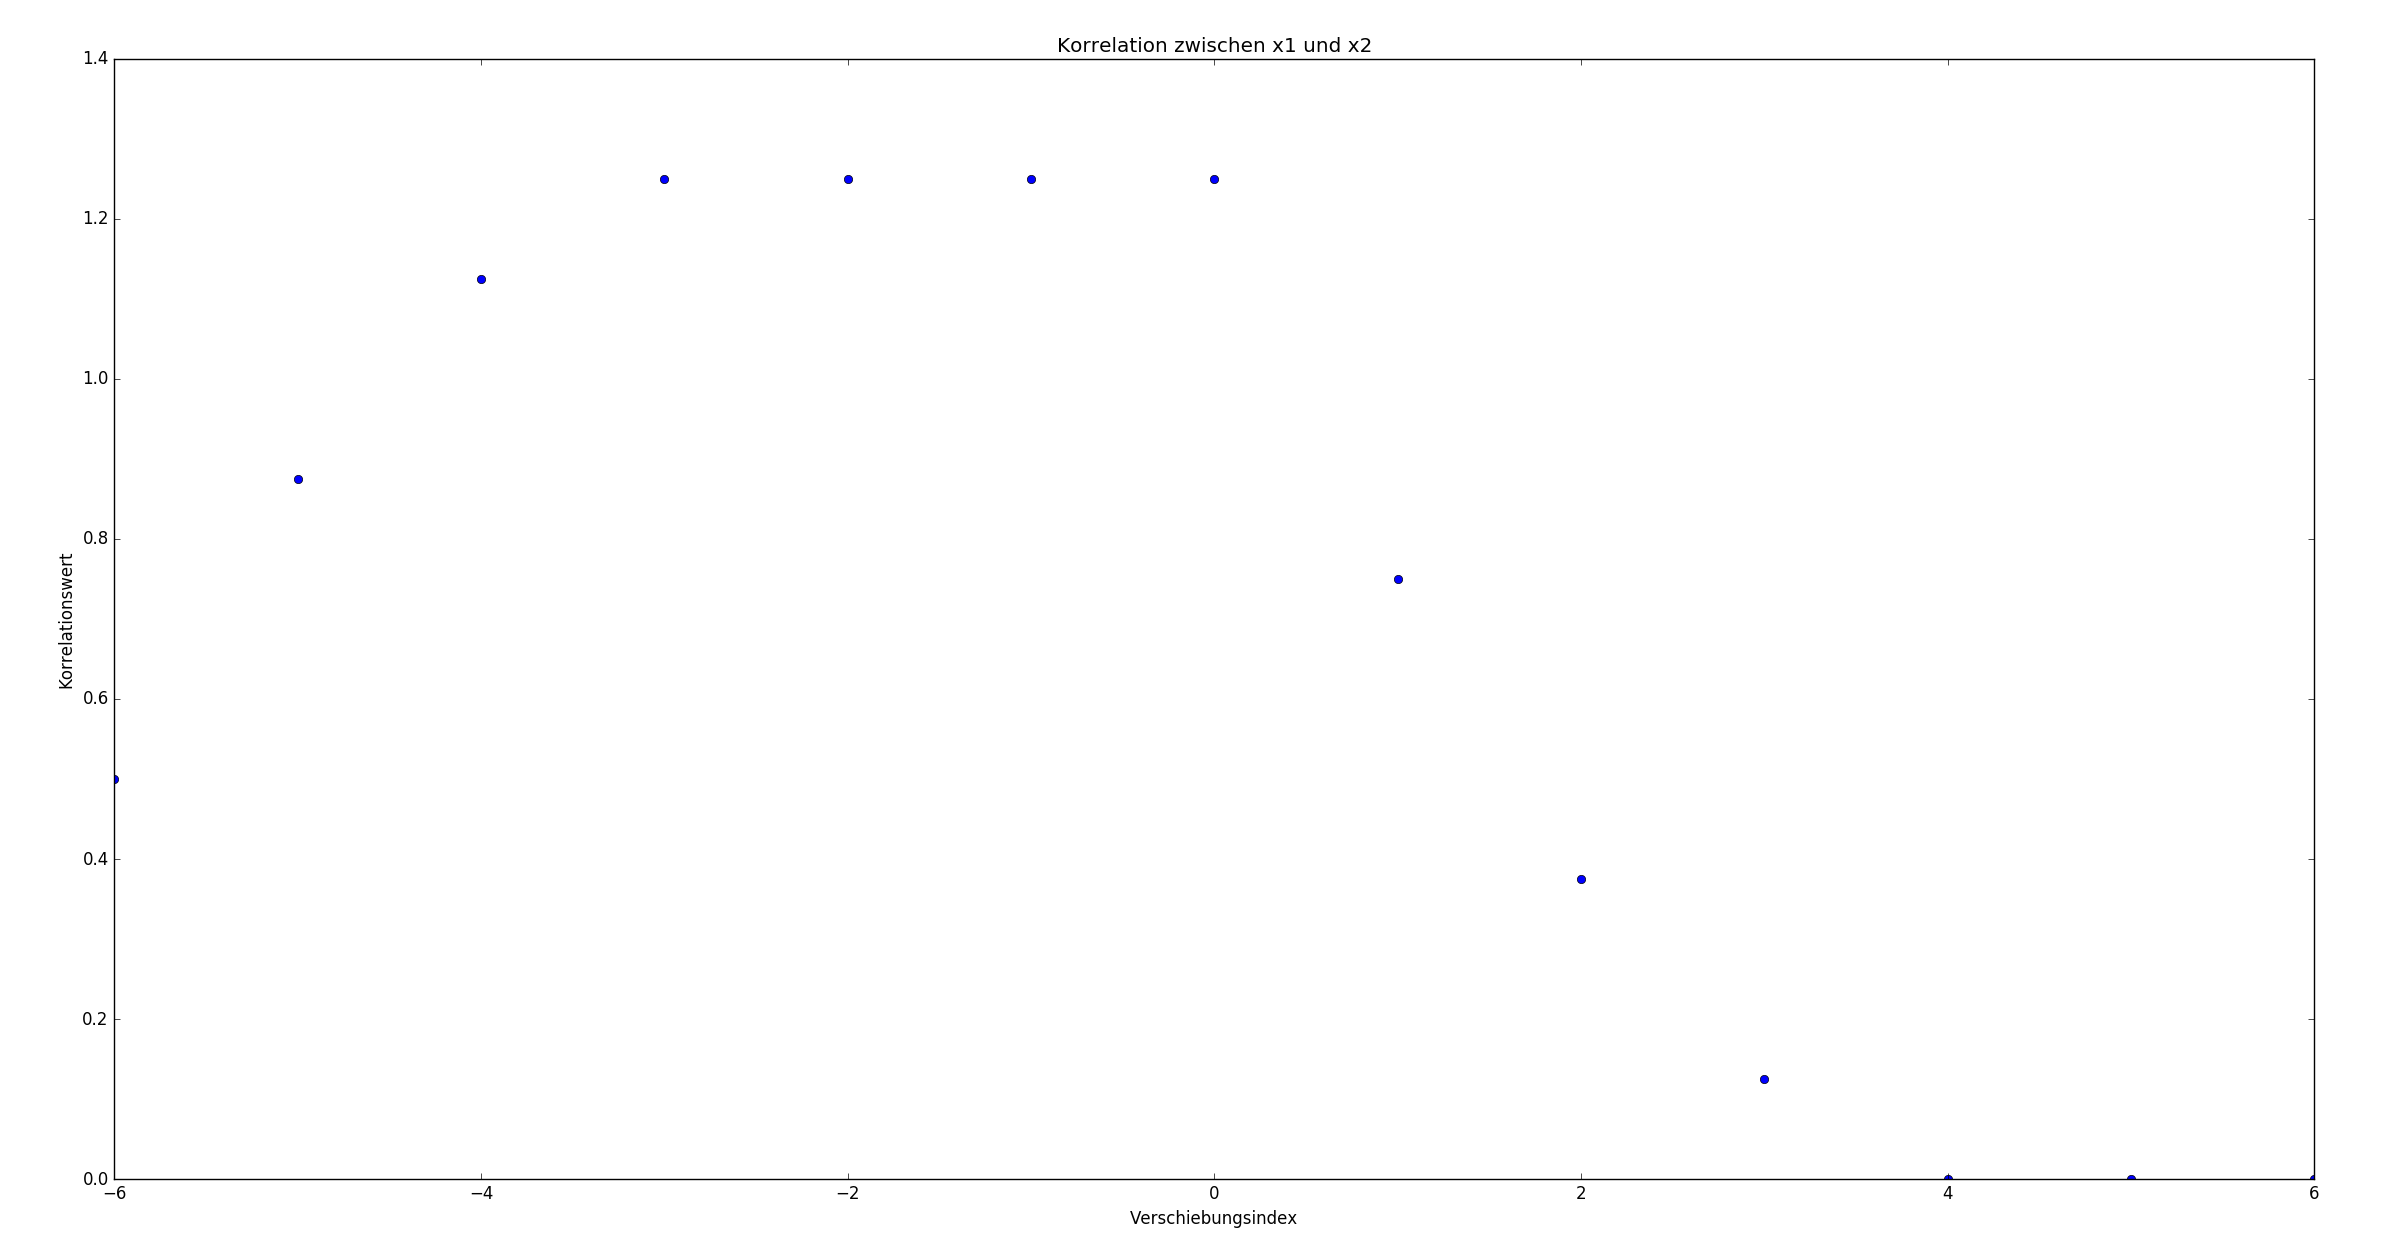
\includegraphics[angle=90, width=0.8\textwidth]{A46.png}
	
\newpage\end{document}